\section{Basic Introduction}

In order to make the zombie epidemic model or the SZR model, a more practical and realistic one, a quarantine model had been developed. The quarantine model was first introduced in [17], and later the perturbation parameter was added in [18]. In this quarantine model, it is assumed that the infected people do not turn into zombies immediately. Rather, before becoming zombies they belong to the exposed category. And in this model, a possibility has been considered to quarantine the people from the exposed category as well as from the zombie category. Hence, it opens up the scope for the introduction and consideration of quarantining people in the model. In [17], the authors estimated that the survival of a healthy human population is not possible according to the model and after some time the healthy human population will go extinct due to this zombie apocalypse. However, in [18], the authors introduced the perturbation parameter in the original model and conjectured the possibility of human survival.  \\


The perturbed SEZQR (susceptible-exposed-zombie-quarantined-removed) model looks like as the following figure ---

\begin{figure}[h]
\centering
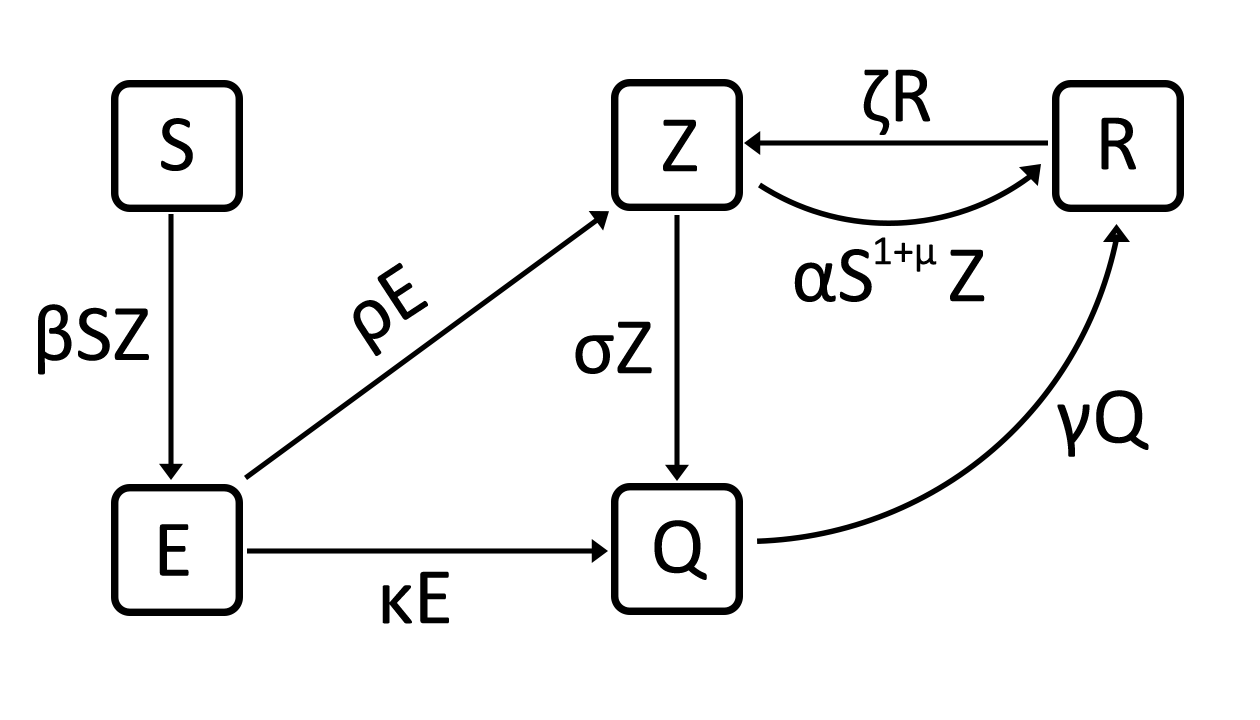
\includegraphics[scale=0.7]{SEZQR.png}
\caption{Perturbed SEZQR Model}
\label{fig:Perturbed SEZQR Model}
\end{figure}

With this perturbed SEZQR model, the transformation of individuals within different compartments is given as follows-
\begin{itemize}
	\item Individuals from susceptible compartment S enter the exposed compartment E at a rate of  \textbeta SZ. This rate depends both on the number of population within the compartments susceptible and zombies.

	\item In the exposed compartment E, individuals are infected with the zombie infection, but are not yet infectious. From this compartment, individuals either enter the zombie compartment Z at a rate of \textrho E or enter the quarantine compartment Q at a rate of \textkappa E.
	
	\item 	In the zombie compartment Z, individuals are infected, infectious and thus hostile. They are capable of spreading the disease among other healthy people. From this compartment, individuals transform to the quarantine category Q at a rate of \textsigma Z. Or, they can also be transformed to removed compartment R (i.e. killed by humans) at a rate of \textalpha S\textsuperscript{(1+\textmu)}Z. Here, in this transformation rate, the perturbation parameter \textmu \ is introduced.
	
	\item In this model, the possibility of quarantining individuals is considered. Hence, here comes the quarantine compartment Q. From this compartment, individuals can be transferred to the removed compartment R at a rate of \textgamma Q.
	
	\item Finally, comes the removed compartment R, where resides all the individuals who either recovered from the compartment Q or are being killed, terminated or neutralized from the compartment Z. However, in this model, no type of immunity is promised or guaranteed. So it is possible that a removed individual can be reinfected or resurrected and can be returned to the zombie compartment again at a rate of \textzeta R.
	
	\item All the entities used in the above transformation rates \textbeta, \textalpha, \textrho, \textkappa, \textsigma, \textgamma,  \textzeta, and the perturbation parameter \textmu \ are positive constants
	
	\item Zombies are removed only through human intervention and interaction. All other natural causes are ignored here.
	
	\item The whole population is homogeneously mixed and every individual has the equal possibility of getting infected.
\end{itemize}

So, this whole perturbed SEZQR model can be summarized as a system of differential equations ---   
\begin{equation}  \label{eq:SEZQR}
\begin{split}
& S' = - \beta SZ \\
& E' = \beta SZ - (\rho + \kappa)E \\
& Z' = \rho E + \zeta R - \sigma Z - \alpha S^{1 + \mu} Z \\
& Q' = \kappa E + \sigma Z - \gamma Q \\
& R' = \alpha S^{1 + \mu} Z + \gamma Q - \zeta R \\
\end{split}
\end{equation}

\pagebreak
\section{Modified Quarantine Model with Perturbation}

However, there are still room for some improvements for the perturbed SEZQR model which was discussed in the previous section, to make it a more pragmatic model. \\

Two modifications can be considered in the existing perturbed SEZQR model. For the first one, the transfer rate of individuals from the zombie compartment Z to the quarantine compartment Q should also depend on the susceptible population S. Because it is logical to theorize that the contribution of the susceptible population is required to quarantine the zombies from the compartment Z to Q. The susceptible people are the only healthy population that are capable of impacting or accelerating the process of quarantining infectious zombies. So, the transfer rate from the zombie compartment Z to the quarantine compartment Q should possibly be \textsigma SZ. \\

Now as for the second modification, it is also logical to consider the possibility of people (or zombies) breaking free from the quarantine compartment Q and joining the zombie compartment Z again. It will not always be possible to keep all the individuals in perfect isolation while in the compartment Q. Some individuals will turn into zombies, or some will break free due to the various reasons, or zombies from the compartment Z can infiltrate the Q compartment and transform some of the individuals from Q compartment into zombies. So this possibility can be examined. The transfer rate of individuals from the compartment Q to the zombie compartment Z can be taken as \textomega Q, where \textomega \ is a positive constant. \\

This newly modified SEZQR model with the existing perturbation parameter can be visualized in the Figure 4.2
\begin{figure}[h]
\centering

\includegraphics[scale=0.9]{SEZQR_mu.png}
\caption{Modified SEZQR Model with Perturbation}
\label{fig:Modified SEZQR Model}
\end{figure}

So, for this newly modified SEZQR model, the system of differential equations will look like --- 
\begin{equation}  \label{eq:ModSEZQR}
\begin{split}
& S' = - \beta SZ \\
& E' = \beta SZ - (\rho + \kappa)E \\
& Z' = \rho E + \zeta R - \sigma SZ - \alpha S^{1 + \mu} Z + \omega Q \\
& Q' = \kappa E + \sigma SZ - \gamma Q - \omega Q \\
& R' = \alpha S^{1 + \mu} Z + \gamma Q - \zeta R \\
\end{split}
\end{equation}

As before, all the variables S, E, Z, Q and R are functions of time, which means that they only change values with respect to the time. And the full size of the population at any given time t, is the grand total of all the individuals from all of the compartments. Which in turn means that, \\

\noindent Total population size, N = S(t) + E(t) + Z(t) + Q(t) + R(t) \\

\noindent So, alternatively, equation (4.2) can be reduced to the following form,

\begin{equation}  \label{eq:ModSEZQR_reduced}
\begin{split}
& S' = - \beta SZ \\
& E' = \beta SZ - (\rho + \kappa)E \\
& Z' = \rho E + \zeta (N - S - E - Z - Q) - \sigma SZ - \alpha S^{1 + \mu} Z + \omega Q \\
& Q' = \kappa E + \sigma SZ - \gamma Q - \omega Q \\
\end{split}
\end{equation}

Also, the whole population is closed. The number of total individuals remains fixed and constant within the given time period t, i.e. $ N^\prime (t) = 0 $. The population is continuous in time. The population is homogeneously mixed and, each and every individual has an equal probability of coming into contact with each other as well as getting infected. \\

In the upcoming sections, this modified SEZQR model will be analyzed mathematically for linear stability. An attempt has been made to find out the condition for disease free equilibrium on the basis of basic reproduction number and the condition for the perturbation parameter \textmu \ to make the modified SEZQR model stable.

\pagebreak
\section{Basic Reproduction Number for Modified \\SEZQR Model}

The expected number of secondary infection cases which are produced by a single or typical infection or infected individual in a completely susceptible population is known as the basic reproduction number \textit{R\textsubscript{0}} [48], [49], [50], [51], [52]. For the modified SEZQR model, this basic reproduction number is the number of individuals who are infected with the zombie disease by a single zombie. In this section, this basic reproduction will be derived based on the modified SEZQR model. But before that, some important terminologies are introduced below. \\

\textbf{Definition 4.1 Spectral Radius: } The largest absolute value of all the eigenvalues (supremum of all the absolute values of the elements in its spectrum) of a square matrix or a bounded linear operator is known as the spectral radius of that matrix or operator [53]. \\

\noindent If X is an $n\times n$ matrix with real or complex elements, and having eigenvalues \textlambda \textsubscript{1}, ..., \textlambda \textsubscript{n}; then the spectral radius \textrho (X) of X is defined as, \\
$
\rho(X)=\max _{1 \leq i \leq n}\left|\lambda_{i}\right|
$
\\

\textbf{Definition 4.2 Jacobian Matrix: } The Jacobian matrix of a vector valued function having several variables is the matrix that contains all the first order partial derivatives of its variables [54], [55]. \\

\noindent For a given set y = f(x), having n equations with n variables x\textsubscript{1}, ..., x\textsubscript{n}, which can be explicitly written as, \\

$
y=\left[\begin{array}{c}
f_{1}(x) \\
f_{2}(x) \\
\vdots \\
f_{n}(x)
\end{array}\right]
$
\\

\noindent Then, the Jacobian matrix is defined as, \\

$
J\left(x_{1}, \ldots, x_{n}\right)=\left[\begin{array}{ccc}
\frac{\partial y_{1}}{\partial x_{1}} & \cdots & \frac{\partial y_{1}}{\partial x_{n}} \\
\vdots & \ddots & \vdots \\
\frac{\partial y_{n}}{\partial x_{1}} & \cdots & \frac{\partial y_{n}}{\partial x_{n}}
\end{array}\right]
$
\\

\textbf{Definition 4.3 Upper Triangular Matrix:  } If all the entries of a square matrix below the main diagonal are zero, then that square matrix is called upper triangular matrix [56]. \\

\noindent A square matrix X is upper triangular if, \\

$
X_{i j}=\left\{\begin{array}{cc}
a_{i j}  \text { for } i \leq j \\
0 \quad \text { for } i>j
\end{array}\right.
$
\\

\noindent Or more explicitly, \\

$
X=\left[\begin{array}{cccc}
a_{11} & a_{12} & \ldots & a_{1 n} \\
0 & a_{22} & \ldots & a_{2 n} \\
\vdots & \vdots & \ddots & \vdots \\
0 & 0 & \ldots & a_{n n}
\end{array}\right]
$
\\
\\

So, now, it is possible to start calculating the value of basic reproduction number, following the methods as described on [18], and some instructions from [60]. As per the system (4.3) and Figure 4.2 of the modified SEZQR model, let us construct a next-generation matrix [57], [58], [59] that focuses only on the compartments that introduce new infections or the spread or transition of infections within the compartments. As such, it is only necessary to focus on the $E^\prime$, $Z^\prime$ and $Q^\prime$ equations. \\

From this, it is now possible to form the new-infection matrix $ \mathcal{F} $ and the transition matrix $ \mathcal{V} $ in such a way that,  \\

[$E^\prime$ $Z^\prime$ $T^\prime$]\textsuperscript{T} = $ \mathcal{F} - \mathcal{V} $ \\

So, for the system (4.3), the new infection matrix $ \mathcal{F} $ and the transition matrix $ \mathcal{V} $ are given by, \\

$
\begin{aligned}
\mathcal{F} &=\left[\begin{array}{c}
\beta S Z \\
0 \\
0
\end{array}\right] \\
\mathcal{V} &=\left[\begin{array}{c}
(\rho+\kappa) E \\
\alpha S^{1+\mu} Z+\sigma S Z-\rho E-\zeta(N-S-E-Z-Q)-\omega Q \\
\gamma Q+\omega Q-\kappa E-\sigma S Z
\end{array}\right]
\end{aligned}
$
\\
\\

Then the basic reproduction number is calculated as per the spectral radius of FV\textsuperscript{-1} , where F and V are the Jacobian matrices of $ \mathcal{F} $ and $ \mathcal{V} $ respectively, which is evaluated at the disease free equilibrium (N, 0, 0, 0, 0). \\

So here we have, \\

$
\begin{aligned}
&F=\left[\begin{array}{ccc}
0 & \beta N & 0 \\
0 & 0 & 0 \\
0 & 0 & 0
\end{array}\right] \\
\end{aligned}
$
\\

and \\

$
\begin{aligned}
&V=\left[\begin{array}{ccc}
(\rho+\kappa) & 0 & 0 \\
(\zeta-\rho) & \alpha N^{1+\mu}+\sigma N+\zeta & \zeta-\omega \\
-\kappa & -\sigma N & \gamma+\omega
\end{array}\right]
\end{aligned}
$
\\

So now the inverse of V, \\

$
V^{-1}=\frac{1}{(\rho+\kappa)\left[(\gamma+\omega)\left(\alpha N^{1+\mu}+\sigma N+\zeta\right)+\sigma N(\zeta-\omega)\right]} \boldsymbol{\cdot} \\
\\
\left[\begin{array}{ccc}
(\gamma+\omega)\left(\alpha N^{1+\mu}+\sigma N+\zeta\right)+\sigma N(\zeta-\omega) & 0 & 0 \\
-[(\zeta-\rho)(\gamma+\omega)+\kappa(\zeta-\omega)] & (\rho+\kappa)(\gamma+\omega) & -[(\rho+\kappa)(\zeta-\omega)] \\
-\sigma N(\zeta-\rho)+\kappa\left(\alpha N^{1+\mu}+\sigma N+\zeta\right) & \sigma N(\rho+\kappa) & (\rho+\kappa)\left(\alpha N^{1+\mu}+\sigma N+\zeta\right)
\end{array}\right]
$
\\
\\

Here the determinant of V, $ det(V) = (\rho+\kappa)\left[(\gamma+\omega)\left(\alpha N^{1+\mu}+\sigma N+\zeta\right)+\sigma N(\zeta-\omega)\right] $ \\

And the adjugate of V, \\

$
det(V)*inv(V) = \\
\left[\begin{array}{ccc}
(\gamma+\omega)\left(\alpha N^{1+\mu}+\sigma N+\zeta\right)+\sigma N(\zeta-\omega) & 0 & 0 \\
-[(\zeta-\rho)(\gamma+\omega)+\kappa(\zeta-\omega)] & (\rho+\kappa)(\gamma+\omega) & -[(\rho+\kappa)(\zeta-\omega)] \\
-\sigma N(\zeta-\rho)+\kappa\left(\alpha N^{1+\mu}+\sigma N+\zeta\right) & \sigma N(\rho+\kappa) & (\rho+\kappa)\left(\alpha N^{1+\mu}+\sigma N+\zeta\right)
\end{array}\right]
$
\\
\\

So, now we can calculate FV\textsuperscript{-1}, \\

$
FV\textsuperscript{-1} = \left[\begin{array}{ccc}
0 & \beta N & 0 \\
0 & 0 & 0 \\
0 & 0 & 0
\end{array}\right] \boldsymbol{\cdot} \frac{1}{(\rho+\kappa)\left[(\gamma+\omega)\left(\alpha N^{1+\mu}+\sigma N+\zeta\right)+\sigma N(\zeta-\omega)\right]}  \boldsymbol{\cdot} \\
\\
\left[\begin{array}{ccc}
(\gamma+\omega)\left(\alpha N^{1+\mu}+\sigma N+\zeta\right)+\sigma N(\zeta-\omega) & 0 & 0 \\
-[(\zeta-\rho)(\gamma+\omega)+\kappa(\zeta-\omega)] & (\rho+\kappa)(\gamma+\omega) & -[(\rho+\kappa)(\zeta-\omega)] \\
-\sigma N(\zeta-\rho)+\kappa\left(\alpha N^{1+\mu}+\sigma N+\zeta\right) & \sigma N(\rho+\kappa) & (\rho+\kappa)\left(\alpha N^{1+\mu}+\sigma N+\zeta\right)
\end{array}\right] \\
\\
$
$
= \frac{-\beta N[(\zeta-\rho)(\gamma+\omega)+\kappa(\zeta-\omega)]}{(\rho+\kappa)\left[(\gamma+\omega)\left(\alpha N^{1+\mu}+\sigma N+\zeta\right)+\sigma N(\zeta-\omega)\right]} \boldsymbol{\cdot} \left[\begin{array}{ccc}
1 & \frac{\beta N(\rho+\kappa)(\gamma+\omega)}{-\beta N[(\zeta-\rho)(\gamma+\omega)+\kappa(\zeta-\omega)]} & \frac{-\beta N(\rho+\kappa)(\zeta-\omega)}{-\beta N[(\zeta-\rho)(\gamma+\omega)+\kappa(\zeta-\omega)]} \\
0 & 0 & 0 \\
0 & 0 & 0
\end{array}\right]
$
\\

This is an upper triangular matrix. So we have the only non-zero eigenvalue, which is the basic reproduction number, \\

\begin{equation}
\textit{R\textsubscript{0}}(\mu) = \frac{-\beta N[(\zeta-\rho)(\gamma+\omega)+\kappa(\zeta-\omega)]}{(\rho+\kappa)\left[(\gamma+\omega)\left(\alpha N^{1+\mu}+\sigma N+\zeta\right)+\sigma N(\zeta-\omega)\right]}
\end{equation} \\

Here , it must be the case that, \\
\begin{equation}
[(\zeta-\rho)(\gamma+\omega)+\kappa(\zeta-\omega)] < 0
\end{equation}\\

Then, with the condition stated in (4.5), \textit{R\textsubscript{0}(\textmu)} will be positive for all values of \textmu.


\pagebreak
\section{Stability Condition for Perturbation Parameter}

In order to determine the value of \textmu \ for which the disease free equilibrium is linearly stable for the modified SEZQR model, we determine the calculation when $ R\textsubscript{0}(\mu) < 1 $. \\

Then we have, \\

$ R\textsubscript{0}(\mu) < 1 \\
$\\
or,
$
\frac{-\beta N[(\zeta-\rho)(\gamma+\omega)+\kappa(\zeta-\omega)]}{(\rho+\kappa)\left[(\gamma+\omega)\left(\alpha N^{1+\mu}+\sigma N+\zeta\right)+\sigma N(\zeta-\omega)\right]} < 1 \\
$
\\
or, 
\begin{equation}
N^{1+\mu}>\frac{\beta N[(\zeta-\rho)(\gamma+\omega)+\kappa(\zeta-\omega)]+(\rho+\kappa)[\sigma N(\zeta-\omega)+(\gamma+\omega)(\zeta+\sigma N)]}{-\alpha(\gamma+\omega)(\rho+\kappa)}
\end{equation}

Since $\alpha(\gamma+\omega)(\rho+\kappa) > 0$, it must be the case that, \\

$\beta N[(\zeta-\rho)(\gamma+\omega)+\kappa(\zeta-\omega)]+(\rho+\kappa)[\sigma N(\zeta-\omega)+(\gamma+\omega)(\zeta+\sigma N)] < 0 $ \\

Which in turn requires that, \\

\begin{equation}
N>\frac{-(\rho+\kappa)[\sigma N(\zeta-\omega)+(\gamma+\omega)(\zeta+\sigma N)]}{\beta[(\zeta-\rho)(\gamma+\omega)+\kappa(\zeta-\omega)]}
\end{equation} 
\\

Finally, in order for the basic reproduction number  $ R\textsubscript{0}(\mu) < 1 $, we have, \\


$ \mu>\frac{\ln \left(\frac{\beta N[(\zeta-\rho)(\gamma+\omega)+\kappa(\zeta-\omega)]+(\rho+\kappa)[\sigma N(\zeta-\omega)+(\gamma+\omega)(\zeta+\sigma N)]}{-\alpha(\gamma+\omega)(\rho+\kappa)}\right)}{\ln (N)}-1 $ \\

\textbf{Theorem 4.1:  } The disease free equilibrium of the modified SEZQR system, satisfying the conditions stated in (4.5) and (4.7), is linearly stable if and only if, \\

\begin{equation}
\mu>\frac{\ln \left(\frac{\beta N[(\zeta-\rho)(\gamma+\omega)+\kappa(\zeta-\omega)]+(\rho+\kappa)[\sigma N(\zeta-\omega)+(\gamma+\omega)(\zeta+\sigma N)]}{-\alpha(\gamma+\omega)(\rho+\kappa)}\right)}{\ln (N)}-1
\end{equation}
\\

It is possible to draw the bifurcation diagram for this modified SEZQR model, with the following set of parameter values. For the estimates of the parameters, those values can be taken from [17], [18]. Also a new value for the parameter \textomega \ is assumed in this table below- \\

\begin{table}[h!]
\centering
 \begin{tabular}{||c c c||} 
 \hline
 Parameter & Description & Estimate \\ [0.5ex] 
 \hline\hline 
 \textbeta & transmission rate for the zombie infection & 0.0095 \\ 
 \textalpha & removal rate of infected zombies & 0.005 \\
 \textzeta & reinfection or resurrection rate for removed individuals & 0.0001 \\
 \textrho & conversion rate from exposed to zombies & 0.005 \\
 \textkappa & quarantine rate of exposed individuals & 0.001 \\
 \textsigma & quarantine rate of zombies & 0.001 \\ 
 \textgamma & removal rate of quarantined individuals & 0.0001 \\ 
 \textomega & conversion rate of quarantined individuals to zombies & 0.009 \\ 
 \textmu & perturbation value & 0.175 \\ [1.5ex] 
 \hline
 \end{tabular}
\caption{Parameter Estimates for the Modified SEZQR Model}
\label{table 4.1}
\end{table}

For the population size of 1000, the bifurcation diagram is given as below,

\begin{figure}[H]
\centering
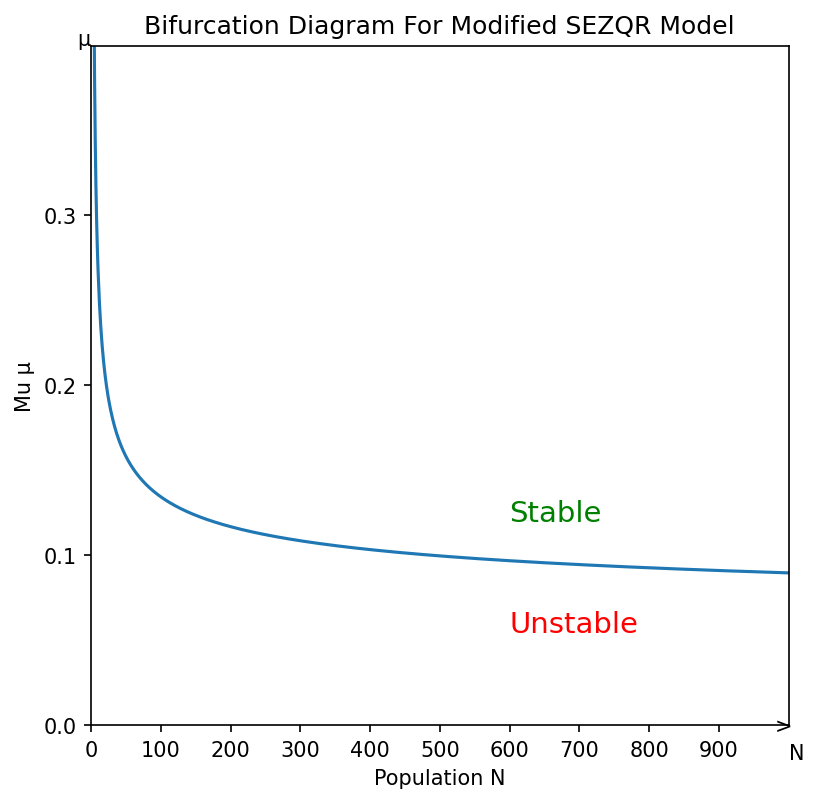
\includegraphics[scale=0.9]{ModifiedSEZQR_Bifurcation.png}
\caption{Bifurcation Diagram for Modified SEZQR Model }
\label{fig:Bifurcation Diagram For Modified SEZQR}
\end{figure}

In the figure 4.3, the bifurcation diagram clearly distinguishes the stable and unstable regions according to the perturbation parameter. \\

And for the given set of values stated on Table 4.1, the conditions stated in (4.5) and (4.7) are also satisfied. So, the Theorem 4.1 states the necessary condition of perturbation parameter to make the modified SEZQR model stable.

\pagebreak
\section{Example of Modified SEZQR Model}

This newly modified SEZQR model with the perturbation parameter, can be numerically solved using an imaginary example, so that it is easier to interpret its behavior. \\

\noindent For this imaginary example, let us consider the following initial conditions--- \\

\noindent The total population size, N = 1000 \\
Initial susceptible population, S(0) = 700 \\
Initial exposed population, E(0) = 100 \\
Initial zombie population, Z(0) = 130 \\
Initial quarantined population, Q(0) = 70 \\
Initial removed population, R(0) = 0 \\
Number of days, t = 1000 \\

And for the other parameter values, those are taken from the Table 4.1. \\

So, now it is possible to solve the system numerically. First the model is solved for 10 days with a step size of 0.1. So that, it is easier to understand and visualize the initial decline of the zombie population. \\

\begin{figure}[H]
\centering
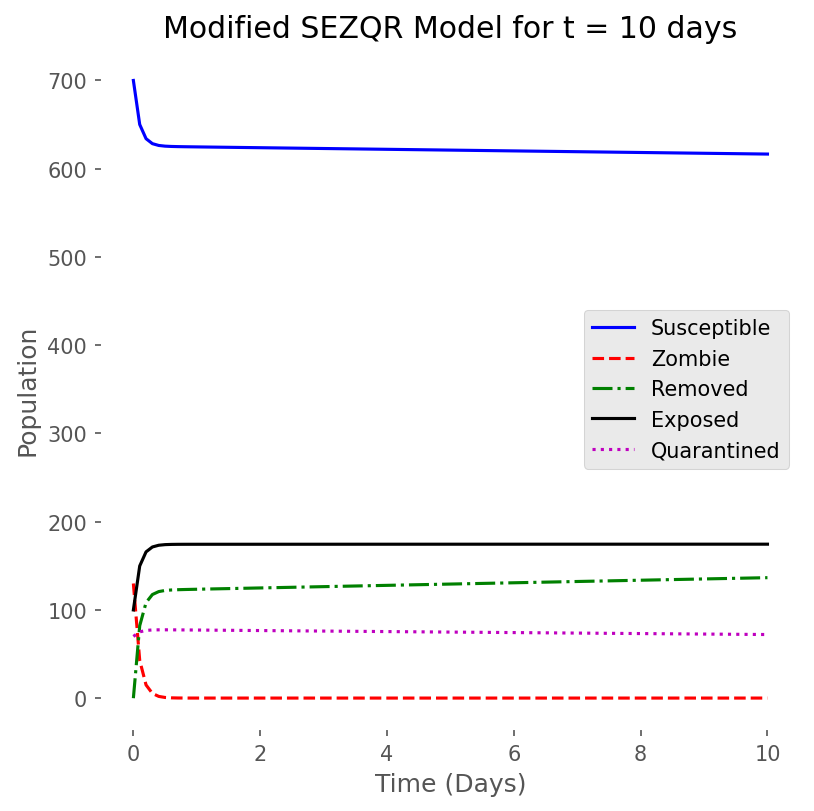
\includegraphics[scale=0.65]{ModifiedSEZQR_10Days.png}
\caption{Modified SEZQR Model for t = 10 days}
\label{fig:Modified SEZQR 10 days}
\end{figure}

And then, the system is solved for t = 1000 days with a step size of 0.1. \\

\begin{figure}[H]
\centering
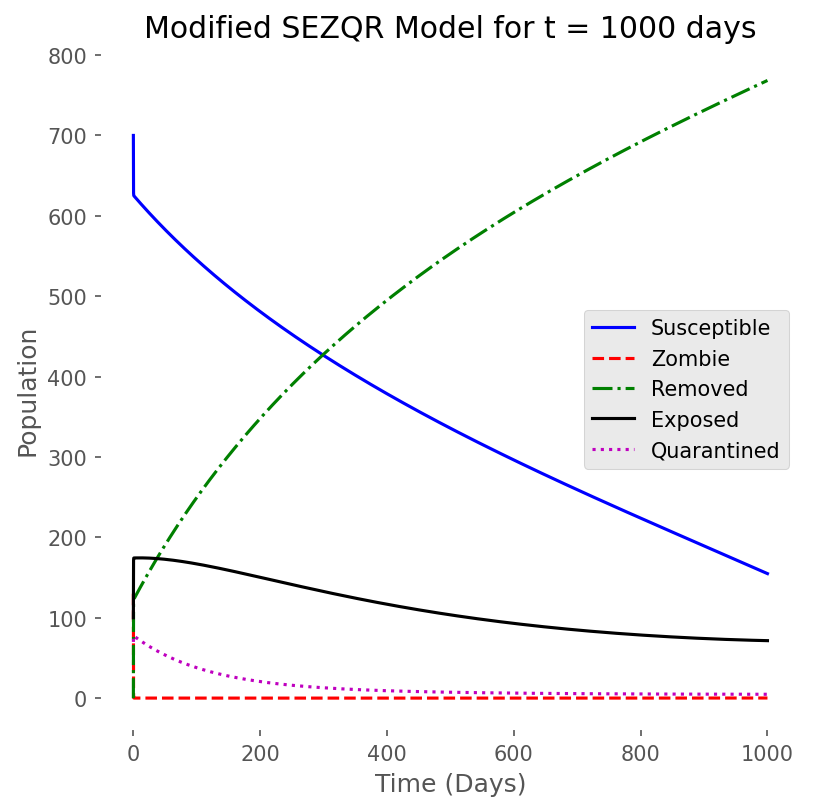
\includegraphics[scale=0.6]{ModifiedSEZQR_1000Days.png}
\caption{Modified SEZQR Model for t = 1000 days}
\label{fig:Modified SEZQR Model 1000 days}
\end{figure}

From the figure 4.5, it is easy to understand that, the removed population R will increase gradually and the zombies will vanish. So it indicates that, the model is stable and a disease free equilibrium is possible in the long run for the perturbation parameter, \textmu \ = 0.175. \\

However, to understand the impact of the perturbation parameter \textmu \ over this modified SEZQR model, the same model is solved again for 1000 days and with a step size of 0.1. But this time, the value of the perturbation parameter \textmu \ is set to zero. 

\begin{figure}[H]
\centering
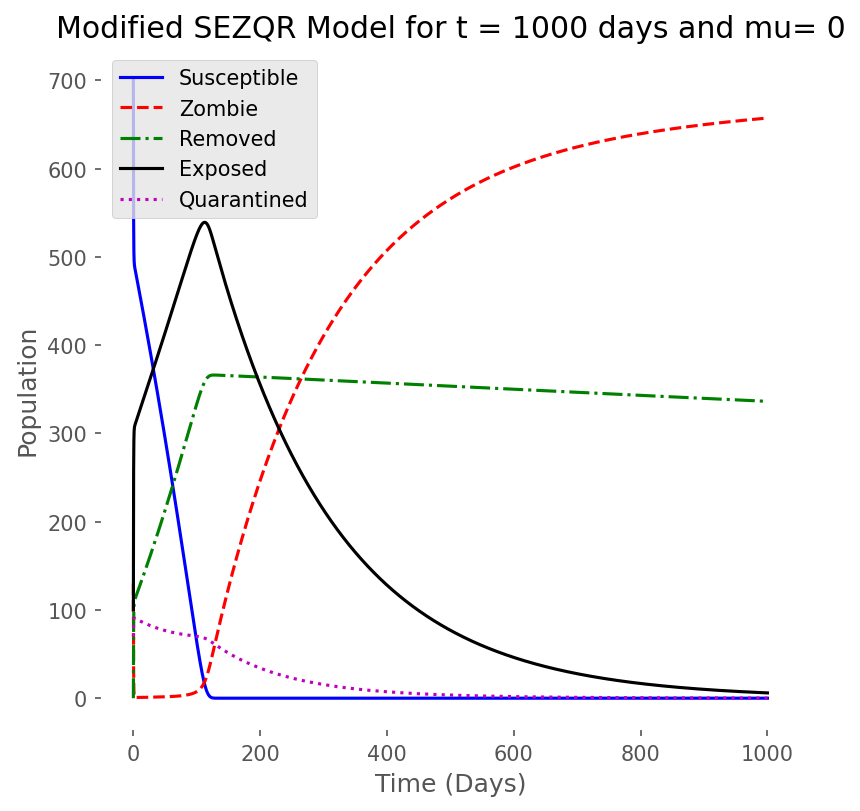
\includegraphics[scale=0.6]{ModifiedSEZQR_1000Days_WithoutMU.png}
\caption{Modified SEZQR Model without Perturbation for t = 1000 days}
\label{fig:Modified SEZQR Model Without Mu}
\end{figure}

From the Figure 4.6, it can be seen that without the perturbation this model is unstable and eventually the zombie population will infect the whole population and cause the extinction of the healthy human population. The susceptible, exposed and quarantined population will vanish in the long run. \\

For the above numerical solutions, the solve\_ivp function [23] was used in the python code. This function uses Runge-Kutta method of order five (RK45) [61], [62], [63], as the integration method. In this method, the error is controlled assuming the accuracy from the fourth-order method, while the steps are taken using the accurate formula of fifth-order. \\

And the phase portrait for the modified SEZQR model with perturbation---\\

\begin{figure}[H]
\centering
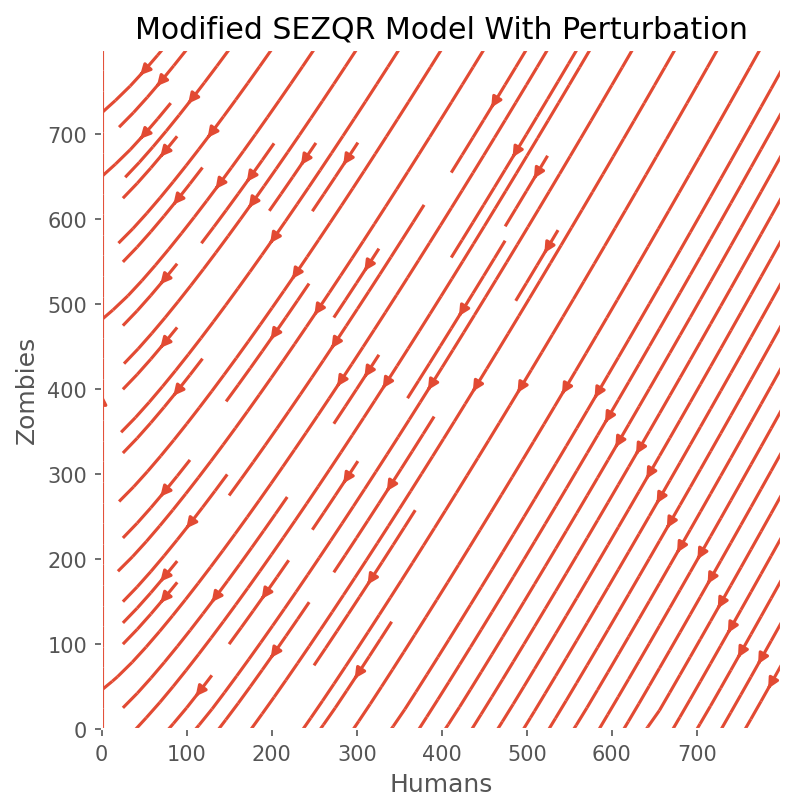
\includegraphics[scale=0.65]{ModifiedSEZQR_PhasePortrait.png}
\caption{Modified SEZQR Model- Phase Portrait}
\label{fig:Modified SEZQR Phase Portrait}
\end{figure}

It is noticeable from the phase portrait also, that with the perturbation, the modified SEZQR model is stable and provides scope for disease free equilibrium. Here, the x-axis (human population) is an attracting set. 

\pagebreak
\section{Effect of Perturbation Parameter on Modified SEZQR Model}

So, to visualize the impact of the perturbation parameter, on the modified SEZQR model and the corresponding zombie population more effectively and efficiently, here another graph is plotted. \\

In this plot, the modified SEZQR model is solved for t = 1000 days, and the population of zombies at the final 1000\textsuperscript{th} day is observed against the increase of the perturbation parameter \textmu. \\

As again, the parameter values are taken from the Table 4.1. And initial conditions are still same as mentioned on the Section 4.5. \\

\begin{figure}[H]
\centering
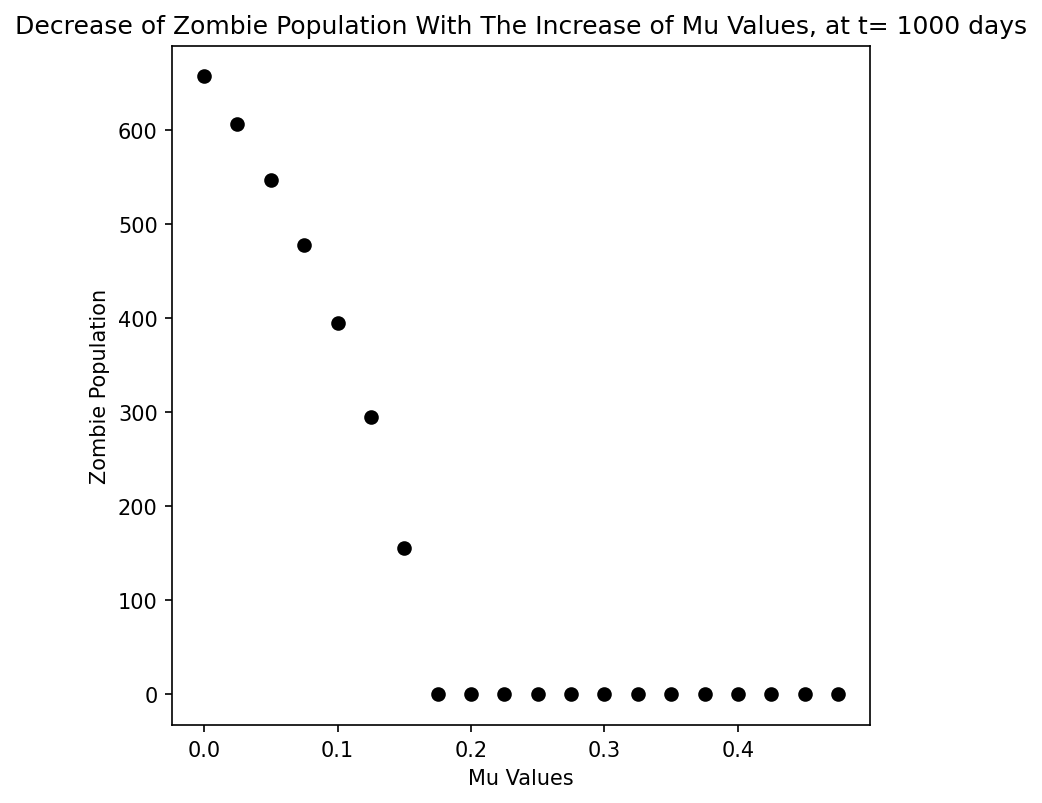
\includegraphics[scale=0.8]{ModifiedSEZQR_Zombie_Mu_Relation.png}
\caption{Modified SEZQR- Relation Between Zombie Population and Perturbation Parameter}
\label{fig:Modified SEZQR Relation}
\end{figure}

As can be seen from the Figure 4.8, the value of zombie population at the final 1000\textsuperscript{th} day position, falls sharply with the increase of perturbation parameter \textmu. The more the value of the perturbation parameter \textmu \ increases, the lower it gets for the zombie population number at the final 1000\textsuperscript{th} day. And at some certain value of perturbation parameter \textmu, the population of zombie totally vanishes at the 1000\textsuperscript{th}  day. \\

Also, if we solve the modified SEZQR system, plot only the zombie population as per different values of perturbation parameter, then another interesting graph can be obtained. \\

\begin{figure}[H]
\centering
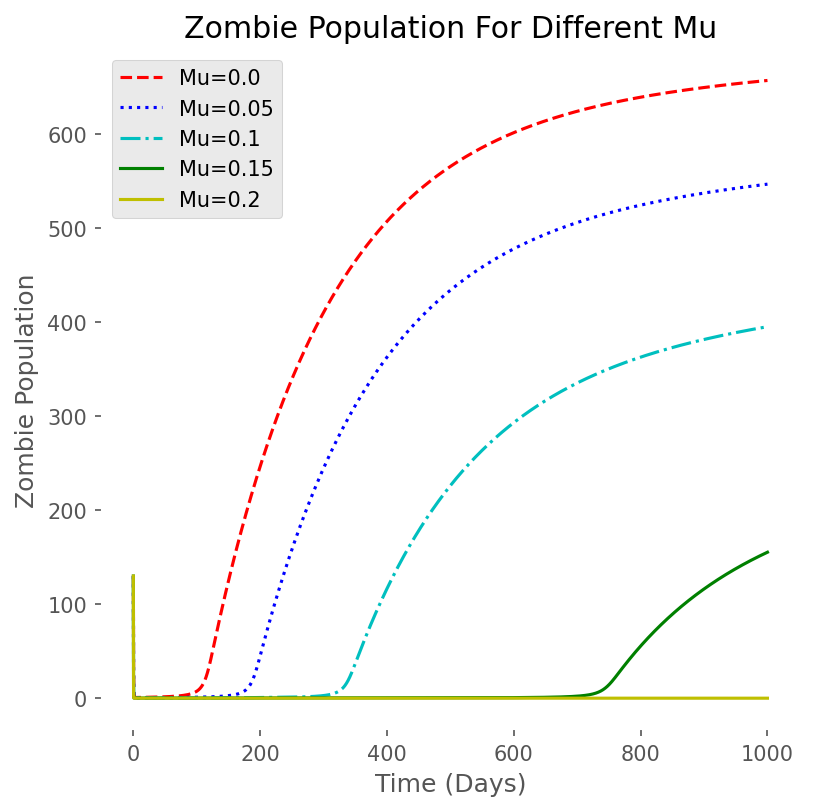
\includegraphics[scale=0.8]{ModifiedSEZQR_Zombie_DifferentMU.png}
\caption{Modified SEZQR- Zombie Population with Different Perturbation Parameters}
\label{fig:Modified SEZQR Relation02}
\end{figure}

In the Figure 4.9, different zombie populations have been plotted for different values of perturbation parameter \textmu. The perturbation parameter \textmu \ value increases from 0.0 until 0.2, with a step size of 0.05. And at the same time, the corresponding zombie population has also been plotted with respect to that particular perturbation parameter \textmu. As the perturbation parameter \textmu \ value increases, the corresponding zombie population also declines gradually. This plot is generated for 1000 days, with the step size of 0.1. \\

So the higher the value of perturbation parameter \textmu \ goes, the faster the zombie population will go extinct. The value of this perturbation parameter \textmu \ depends on the human capacity and skills to remove and neutralize zombies in the real world.

\pagebreak
\section{Comparison of Models}

In this section, some basic comparisons will be made for the Modified SEZQR model, with the perturbed SEZQR model from [18], which was discussed in the Section 4.1 of this chapter. The perturbed SEZQR model is already depicted in Figure 4.1 and the related system of differential equations was expressed in equation (4.1). \\

In the Theorem 2 of [18], the condition for the perturbation parameter of the SEZQR model, to introduce a disease-free equilibrium is defined as, \\

\begin{equation}
\mu>\frac{\ln \left(\frac{\beta N(\zeta \kappa+\gamma(\zeta-\rho))+(\rho+\kappa)(\zeta \sigma+\gamma(\zeta+\sigma))}{-\alpha \gamma(\rho+\kappa)}\right)}{\ln (N)}-1
\end{equation}

So, according to this condition, the bifurcation diagram for the SEZQR model looks like the figure given below. The parameter values are same as of Table 4.1 and the population size is 1000. \\

\begin{figure}[H]
\centering
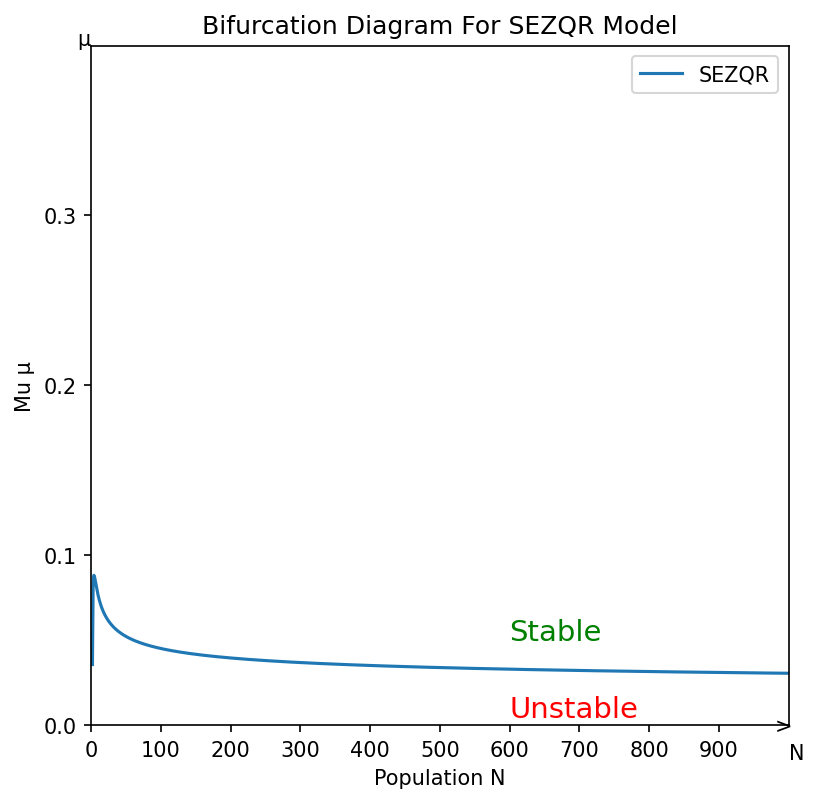
\includegraphics[scale=0.8]{SEZQR_Birfurcation.png}
\caption{Bifurcation Diagram for SEZQR Model}
\label{fig:Bifurcation SEZQR}
\end{figure}

Now, the bifurcation diagrams for both the SEZQR model and the modified SEZQR model are plotted within a single frame, \\

\begin{figure}[H]
\centering
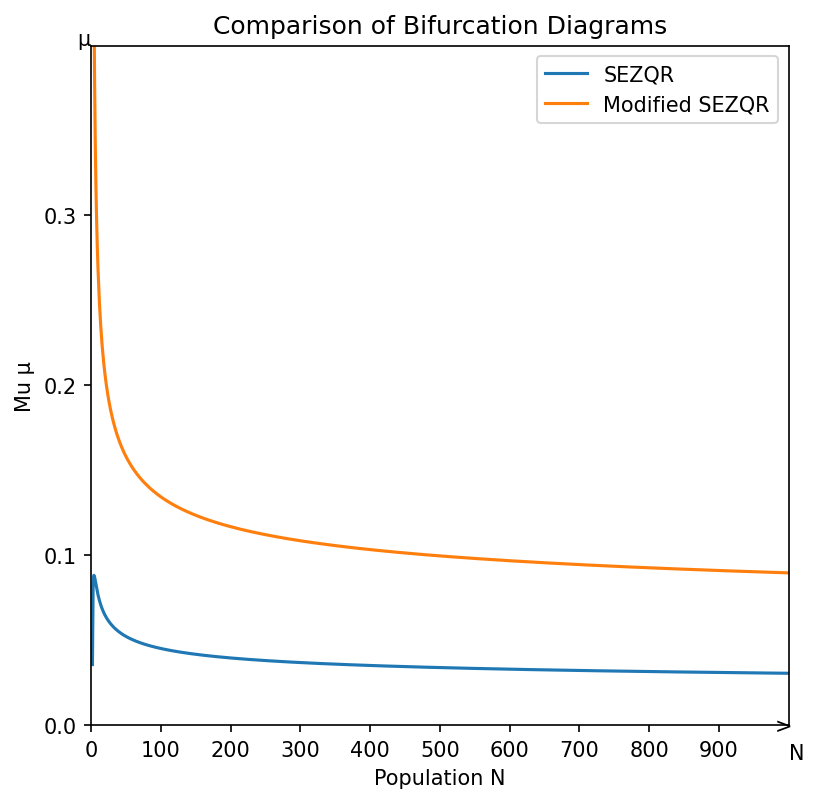
\includegraphics[scale=0.8]{Bifurcation_Comparison.png}
\caption{Bifurcation Diagrams Comparison}
\label{fig:Bifurcation Comparison}
\end{figure}

In the Figure 4.11, the bifurcation diagram for the modified SEZQR model is plotted using a yellow line, while the bifurcation line for the regular perturbed SEZQR model uses a magenta line. Any area above the curve line is stable for that line, and the area below the curve line marks the unstable region for that line. \\

It is easily visible that, the stability region for the perturbation parameter \textmu \ of the regular SEZQR model is bigger than the stability region of the modified SEZQR model. The modified SEZQR model has a bigger unstable region for the perturbation parameter \textmu. The possibilities of individuals breaking free from the quarantine compartment Q and returning to the zombie compartment Z as well as the influence of the susceptible population in quarantining zombies from the compartment Z to Q, that were introduced in the modified SEZQR model have caused the change in the region of stability for this model. \\

Also, if we numerically solve the SEZQR model for 1000 days with the same set of data used in the example of Section 4.5 of this chapter and compare it side by side with the solution of the modified SEZQR model (from the Figure 4.5), we will get the following scenario, \\

\begin{figure}[H]
\centering
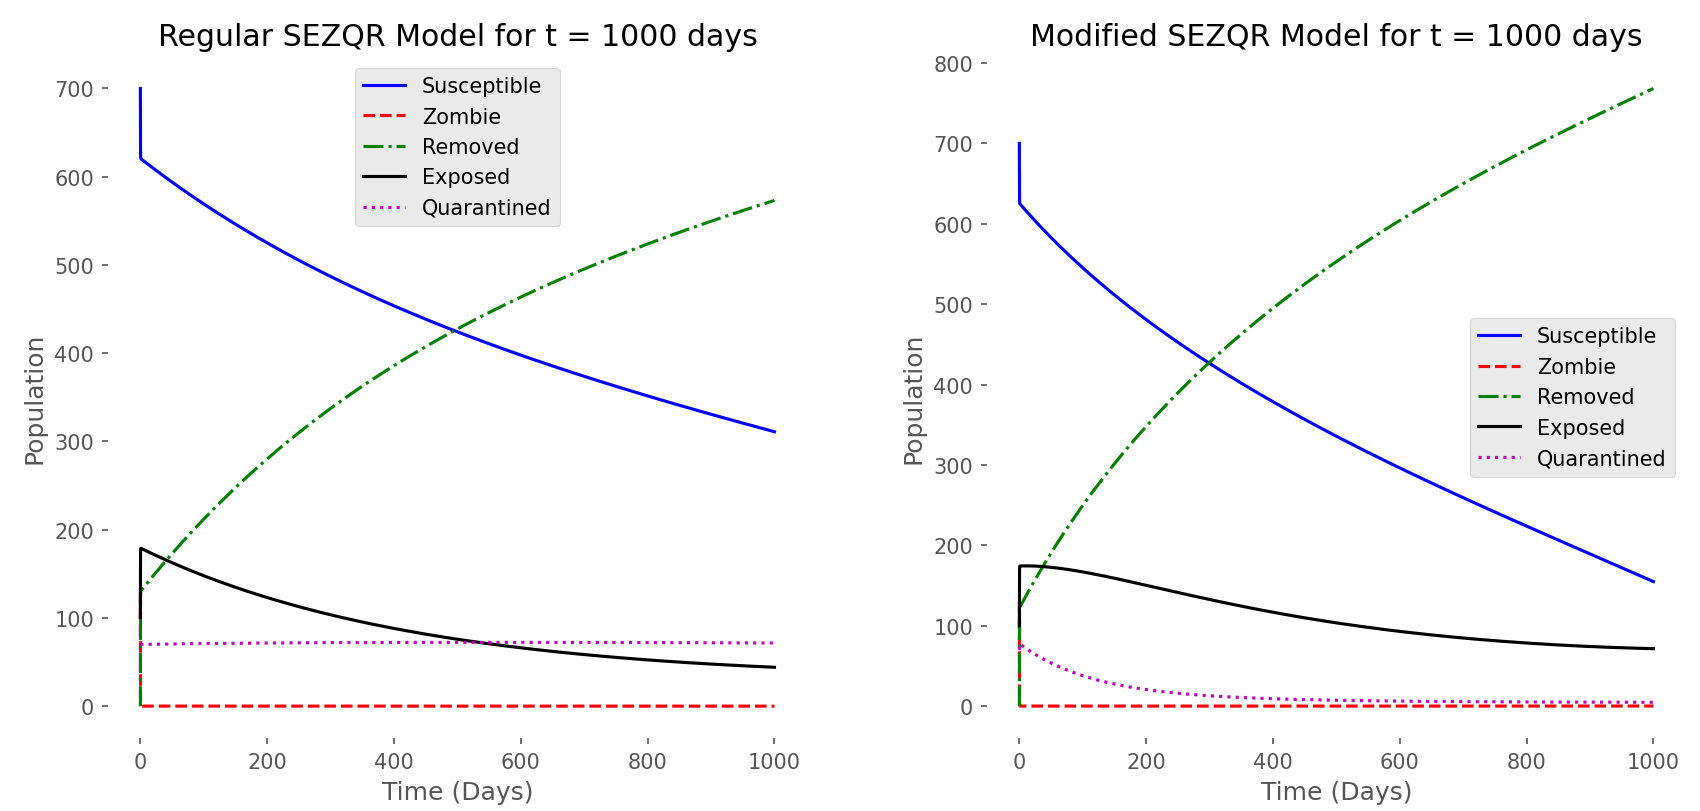
\includegraphics[scale=0.5]{Solution_Comparison.png}
\caption{Solution Comparison- SEZQR vs. Modified SEZQR}
\label{fig:Solution Comparison}
\end{figure}

In the Figure 4.12, both the solutions are plotted using the same set of data and for 1000 days. It can be seen that, the susceptible population line for the modified SEZQR model falls rapidly when compared to the susceptible line of the regular SEZQR model. On the other hand, the removed population line on the modified SEZQR model rises faster than that of the regular SEZQR model. While the zombie population lines remain almost similar for both of the graphs, there are some changes in behavior for the exposed and quarantined population lines. In the modified SEZQR model, the quarantined population line also goes downward gradually. The changes introduced in the modified SEZQR model have caused the dynamics of this model to act differently than the regular perturbed SEZQR model. \\

\pagebreak
\section{Special Case 01: Exposed = 0}

Let us consider a special scenario, in which E = 0. That means, there is no individual in the exposed population. As such, no new individual can be turned into zombies Z or can be transferred to the quarantined compartment Q from the exposed compartment E. \\

Also it is important to note that, in the modified SEZQR model, the transfer rates \textalpha S\textsuperscript{(1+\textmu)}Z (from compartment Z to R) and \textsigma SZ (from compartment Z to Q) are still depending on the initial susceptible population S. But as there is no exposed population E, the original susceptible population S is also absent in the field. So it is no longer possible for the susceptible population S to impact the transfer rates of zombies Z. \\

So, now the population transformation dynamics will be confined within the compartments Z, Q and R. This can be visualized as below-- \\

\begin{figure}[H]
\centering

\includegraphics[scale=1.4]{SpecialCase01.png}
\caption{Special Case 01}
\label{fig:Special Case 01}
\end{figure}


And, the new set of differential equations will look like, with E being 0 and S being absent, \\

\begin{equation}
\begin{aligned}
&Z^{\prime}=\zeta R+\omega Q \\
&Q^{\prime}=-\gamma Q-\omega Q \\
&R^{\prime}=\gamma Q-\zeta R
\end{aligned}
\end{equation}

Which can be reduced in the short form as below, \\

\begin{equation}
\begin{aligned}
&Z^{\prime}=\zeta (N - Z - Q)+\omega Q
\end{aligned}
\end{equation}

\begin{equation}
\begin{aligned}
&Q^{\prime}=-\gamma Q-\omega Q
\end{aligned}
\end{equation}

Here, equation (4.12), is a first order linear ordinary differential equation. Solving this equation, we get the exact solution, \\

\begin{equation}
Q=c_{1} \mathrm{e}^{-(\gamma+\omega) t}
\end{equation}

Where, c\textsubscript{1} is a constant. \\

Putting this value in the equation (4.11), we get, \\

\begin{equation}
\begin{aligned}
&Z^{\prime}=\zeta N-\zeta Z+(\omega-\zeta) Q \\
\text {or}, \ &Z^{\prime}=-\zeta Z+f(t)
\end{aligned}
\end{equation}

Where, 
\begin{align*} f(t)& = \zeta N + (\omega - \zeta)Q \\
 & = \zeta N + (\omega - \zeta)(c_{1} \mathrm{e}^{-(\gamma+\omega) t}) \end{align*}

Equation (4.14) is a nonhomogeneous linear differential equation. \\

The system of equations (4.10) can be solved numerically, with the same set of parameter values mentioned in Table 4.1 and initial conditions discussed in the example of Section 4.5 of this chapter. \\

\begin{figure}[H]
\centering
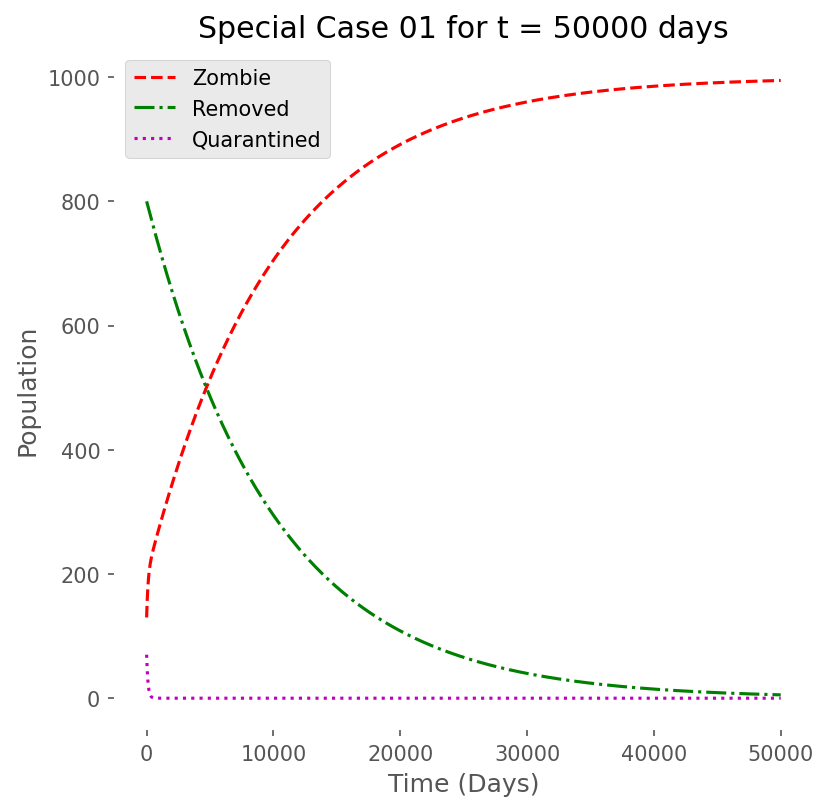
\includegraphics[scale=0.8]{SpecialCase01_Solution.png}
\caption{Special Case 01 Numerical Solution}
\label{fig:Special Case 01 Solution}
\end{figure}

Here the system is solved for 50,000 days, with a step size of 1. It can be seen that, in the long run the whole population turns into zombies, and the removed population as well as the quarantined population all disappear eventually. The perturbation parameter is absent from the equations, so there is no way to impact or perturb the dynamics of the model here. \\

This type of scenario (that the exposed population being zero) is only possible when all the individuals from the susceptible S population are already put into the Z or Q compartments and no new human is left for interaction or infection. \\

Or, the Z, Q and R categories are being isolated in such a closed system that they cannot interact with any new population. For example these categories can be put into a location or city which is totally disconnected or cut off with the rest of the country/world.  \\

\pagebreak
\section{Special Case 02: Zombies = 0}

For the special case 02, let us consider the circumstance when the population of Z compartment turns into zero. It means that there are no new zombies left to contaminate or infect new people in the susceptible population S (because the transfer rate \textbeta SZ and \textalpha S\textsuperscript{(1+\textmu)}Z will be zero, as Z = 0). As such, the population of the compartments E, Q  will gradually turn into zero and the whole system will be stable again with the healthy people only. \\

So, the new system will look like--- \\

\begin{equation}
\begin{aligned}
&S^{\prime}=0 \\
&E^{\prime}=-(\rho+\kappa) E \\
&Z^{\prime}=\rho E+\zeta R+\omega Q \\
&Q^{\prime}=\kappa E-\gamma Q-\omega Q \\
&R^{\prime}=\gamma Q-\zeta R
\end{aligned}
\end{equation}

This system can be reduced in the form given below, \\

\begin{equation}
\begin{aligned}
&E^{\prime}=-(\rho+\kappa) E \\
&Z^{\prime}=\rho E+\zeta (N - S - E - Q)+\omega Q \\
&Q^{\prime}=\kappa E- (\gamma + \omega) Q \\
\end{aligned}
\end{equation}

But it is also important to note that, here as all the zombies have vanished (Z = 0), so it is not possible to produce new zombies or spread the infection anymore. As such the transfer rates \textzeta R, \textomega Q, \textgamma Q, \textrho E, \textkappa E will turn into meaningless entities. So it is not logical to model or simulate this system of differential equations, as it is no longer relevant or realistic. \\

As all the zombies have been vanished, the whole population will be filled with healthy people only and no new infection is possible. Thus, it is no longer possible or sensical to transfer individuals within the given E, Z, Q, R compartments. These compartments do not exist anymore.




